\documentclass{beamer}

\usepackage[utf8]{inputenc}
\usepackage[english, russian]{babel}

\usetheme{Madrid}


\title[Эффекты самоорганизации в рекомендательных системах]{Эффекты самоорганизации в рекомендательных системах}
\author{Дементьев Сергей}
\institute[МФТИ]{Московский физико-технический институт}
\date{17 апреля, 2025} % Убираем дату

\setbeamertemplate{footline}{%
  \leavevmode%
  \hbox{%
  \begin{beamercolorbox}[wd=\paperwidth,ht=2.25ex,dp=1ex,left]{author in head/foot}%
    \usebeamerfont{author in head/foot}\hskip1em \insertshortauthor\ (\insertshortinstitute) \quad \textcolor{gray}{|} \quad \insertshorttitle\hskip1em%
    \textcolor{gray}{|}\usebeamerfont{page number in head/foot}\hfill\insertframenumber{} / \inserttotalframenumber\hskip1em%
  \end{beamercolorbox}}%
  \vskip0pt%
}


\begin{document}

\begin{frame}
    \titlepage
\end{frame}

\begin{frame}{Цель исследования}
    \begin{itemize}
        \item Если не учитывать эффекты самоорганизации в рекомендательных системах, то можно получить деградацию модели
        \item Также можно получить смещение распределения пользователей – останутся только те, кому нравится именно этот рекомендательный алгоритм. (петля обратной связи)
        \item Но если мы знаем какие параметры влияют на возникновение петли и каков характер этой связи, то \textbf{мы можем контролировать появление самоорганизации в системе}.
    \end{itemize}
\end{frame}

\begin{frame}{Проблема}
  \begin{itemize}
    \item \textbf{Существующие компоненты системы:}
      \begin{itemize}
        \item \textbf{Алгоритм рекомендаций ($a_{rec}$):} отвечает за формирование персональных рекомендаций товаров пользователям.
        \item \textbf{Алгоритм выбора пользователя ($a_{choice}$):} моделирует, на какие из предложенных рекомендаций пользователь вероятно отреагирует.

        \item \textbf{Генераторы новых пользователей ($userGAN$) и новых товаров($itemGAN$):} алгоритмы, способный изменять распределения объектов: как удаляют, так и добавляют новых.
      \end{itemize}
    \item \textbf{Динамика распределений:}
      \begin{itemize}
        \item В процессе взаимодействия происходит изменение распределения по некоторому закону, который мы и хотим исследовать.
          \begin{itemize}
            \item $\mathbf{D}$ – оператор эволюции распределения. 
            
            \item Распределение пользователей: $f_u^t$ и  $\mathbf{D}f_u^t = f_u^{t+1}$
            \item Распределение товаров: $f_i^t$ и  $\mathbf{D}f_i^t = f_i^{t+1}$
          \end{itemize}
      \end{itemize}
  \end{itemize}
\end{frame}

%\begin{frame}{Гипотезы}
 %   На возникновение петли в рекомендательной системе влияет:
    
  %  \begin{itemize}
   %     \item Размерность данных, а также наличие шума в них. 
    %    \item Тип функциональной зависимости удовлетворенности от рекомендаций со временем.
        
     %   \item Количество информации, которое есть в распоряжении алгоритма рекомендаций.
%    \end{itemize}
%\end{frame}


\begin{frame}{Гипотезы}
  На возникновение петли обратной связи в рекомендательной системе влияют следующие ключевые факторы:
  \begin{itemize}
    \item \textbf{Характеристики данных:}
      \begin{itemize}
        \item \textbf{Размерность данных:} чем выше размерность, тем сложнее может быть обнаружение истинных зависимостей.
        \item \textbf{Наличие шума:} высокий уровень шума может искажать сигналы и приводить к неверным выводам.
      \end{itemize}
    \item \textbf{Функция удовлетворенности:}
      \begin{itemize}
        \item \textbf{Тип зависимости:} характер изменения удовлетворенности пользователей от рекомендаций с течением времени (например, линейная, убывающая, насыщающая).
      \end{itemize}
    \item \textbf{Информационная обеспеченность алгоритма:}
      \begin{itemize}
        \item \textbf{Объем доступной информации:} количество данных о пользователях, товарах и их взаимодействиях, которое использует алгоритм рекомендаций.
      \end{itemize}
  \end{itemize}
\end{frame}

% Слайд из файла пользователя (обязательный)
\begin{frame}{Как определить, что петля есть?}

  \boxed{\textbf{Определение:}}
  \vspace{0.3em}
  
  Пусть $A_t$ – рекомендации системы, а $R_t$ – оценки пользователей на шаге $t$. Если:

  \[
      P(\{ R_s \}_{s=1}^t \mid \{ A_s \}_{s=1}^t) \neq \prod_{s=1}^t P(R_s \mid A_s)
  \]
  Тогда мы считаем, что в системе возникает петля обратной связи. 
  
  \vspace{1em} % Добавляем немного вертикального пространства для лучшей читаемости

  \boxed{\textbf{Численный критерий возникновения петли:}}
  \vspace{0.3em}
  
  Пусть $F, \mathcal{L}$ – функционал качества и функция Лосса
  
  $\exists t_0, \Delta \in \mathbb{N}: \quad \mathcal{L}(R_{t+1}, A_{t+1}) < \mathcal{L}(R_t, A_t)$, а также  $F(R_{t+1}, A_{t+1}) < F(R_t, A_t) \quad   \forall t \in \overline{t_0, \ldots t_0 + \Delta - 1}$

\end{frame}

\begin{frame}{Модель}
    \begin{itemize}
         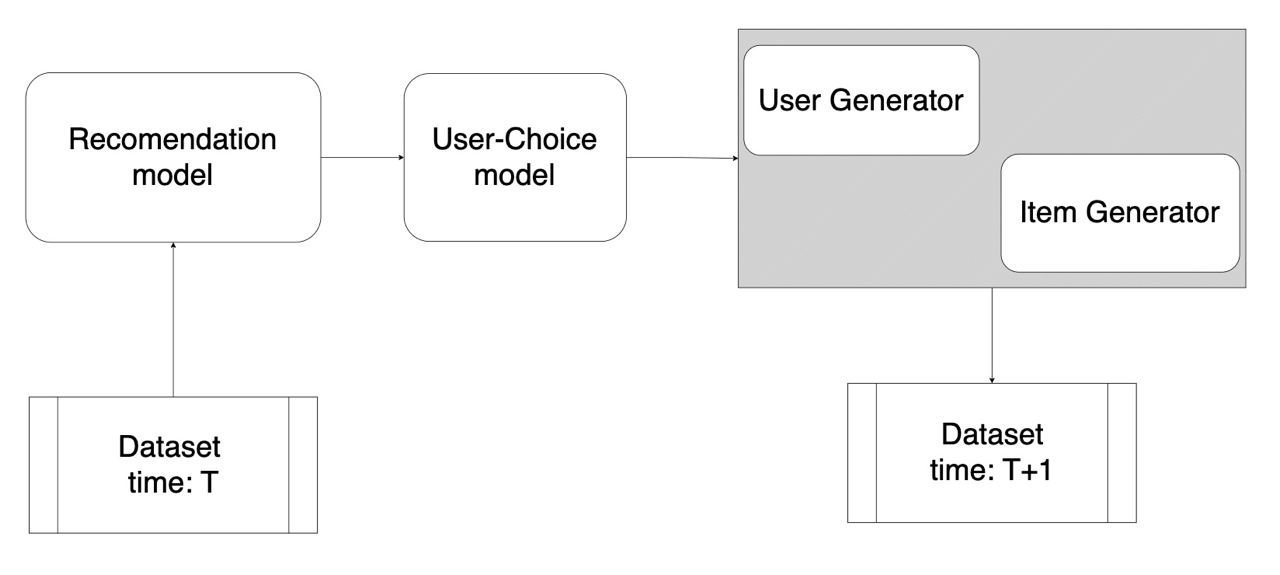
\includegraphics[width=0.9\textwidth]{model.png}
    \end{itemize}
\end{frame}

\begin{frame}{Эксперимент и его результаты}

    \begin{itemize}
        
         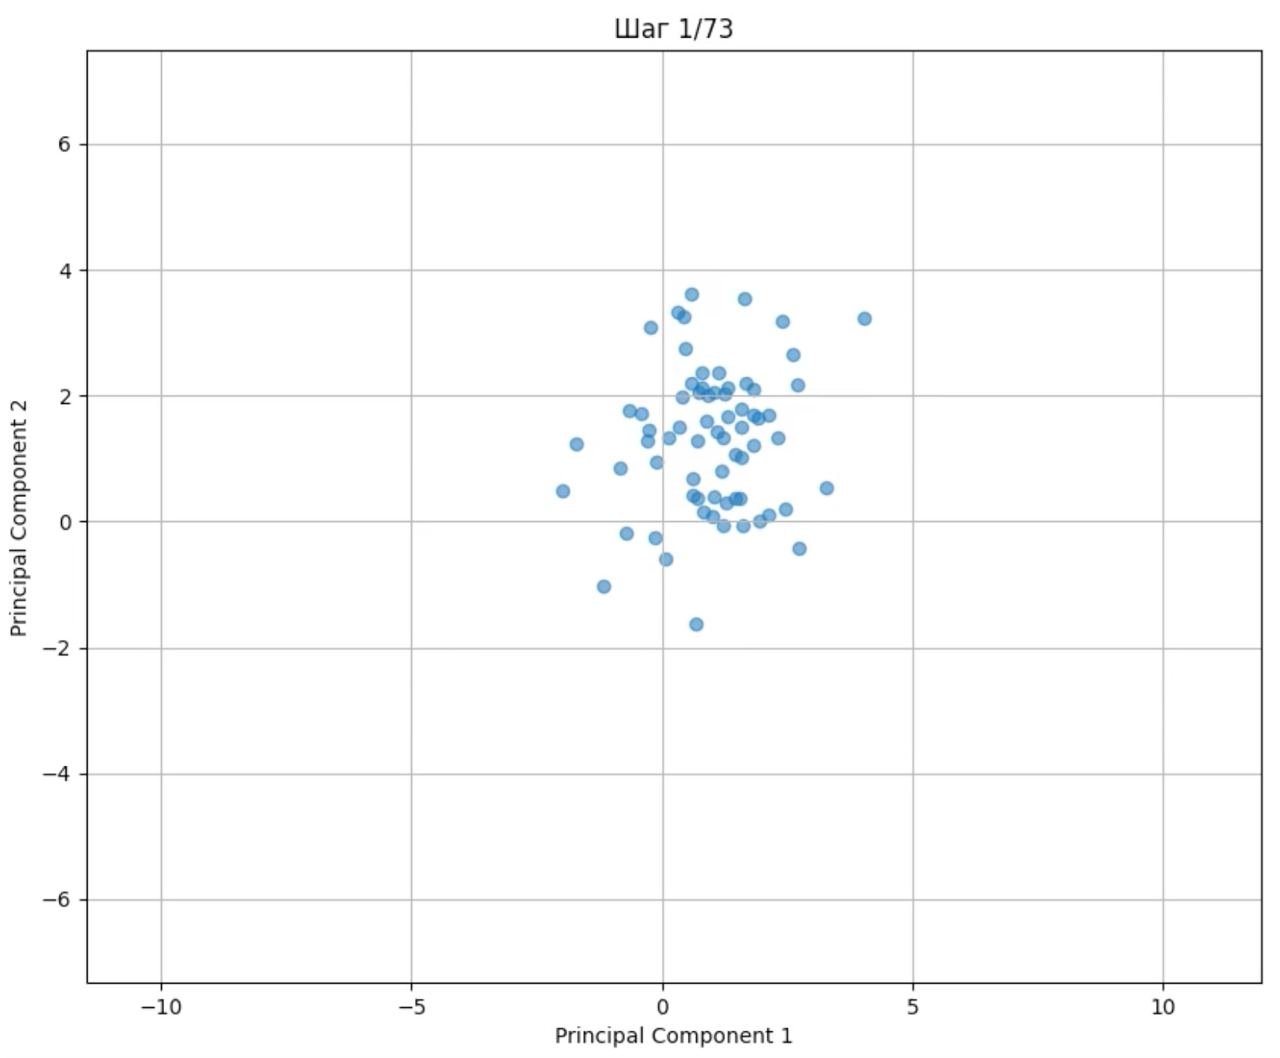
\includegraphics[width=0.4 \textwidth]{user_loop_1.png}


         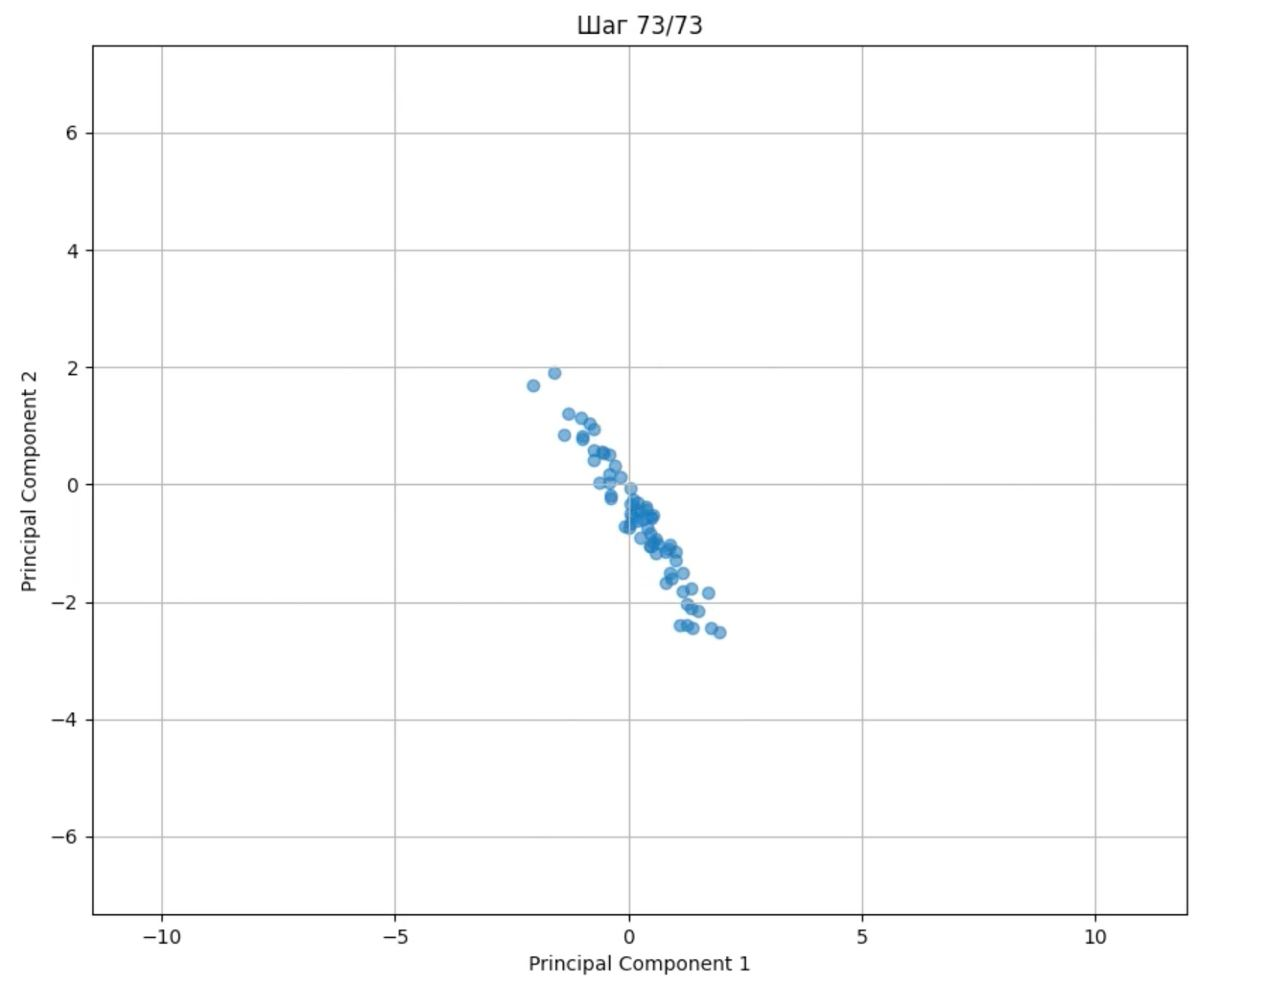
\includegraphics[width=0.43 \textwidth]{user_loop_2.png}

    \end{itemize}
    
\item {Скрытая петля положительной обратной связи }
\end{frame}


\begin{frame}{Эксперимент и его результаты}

    \begin{itemize}
        
         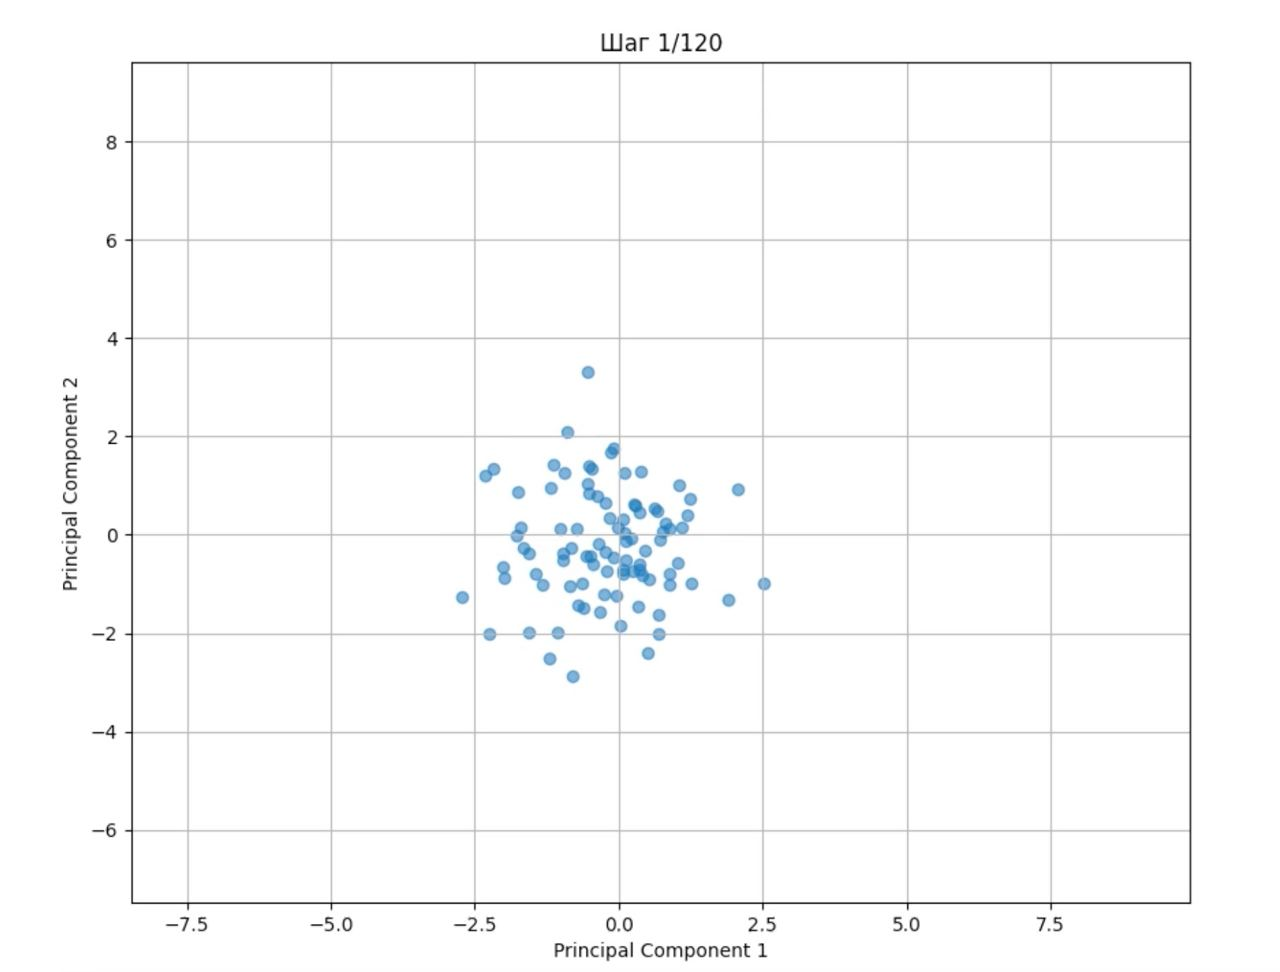
\includegraphics[width=0.4 \textwidth]{user_stable_1.png}


         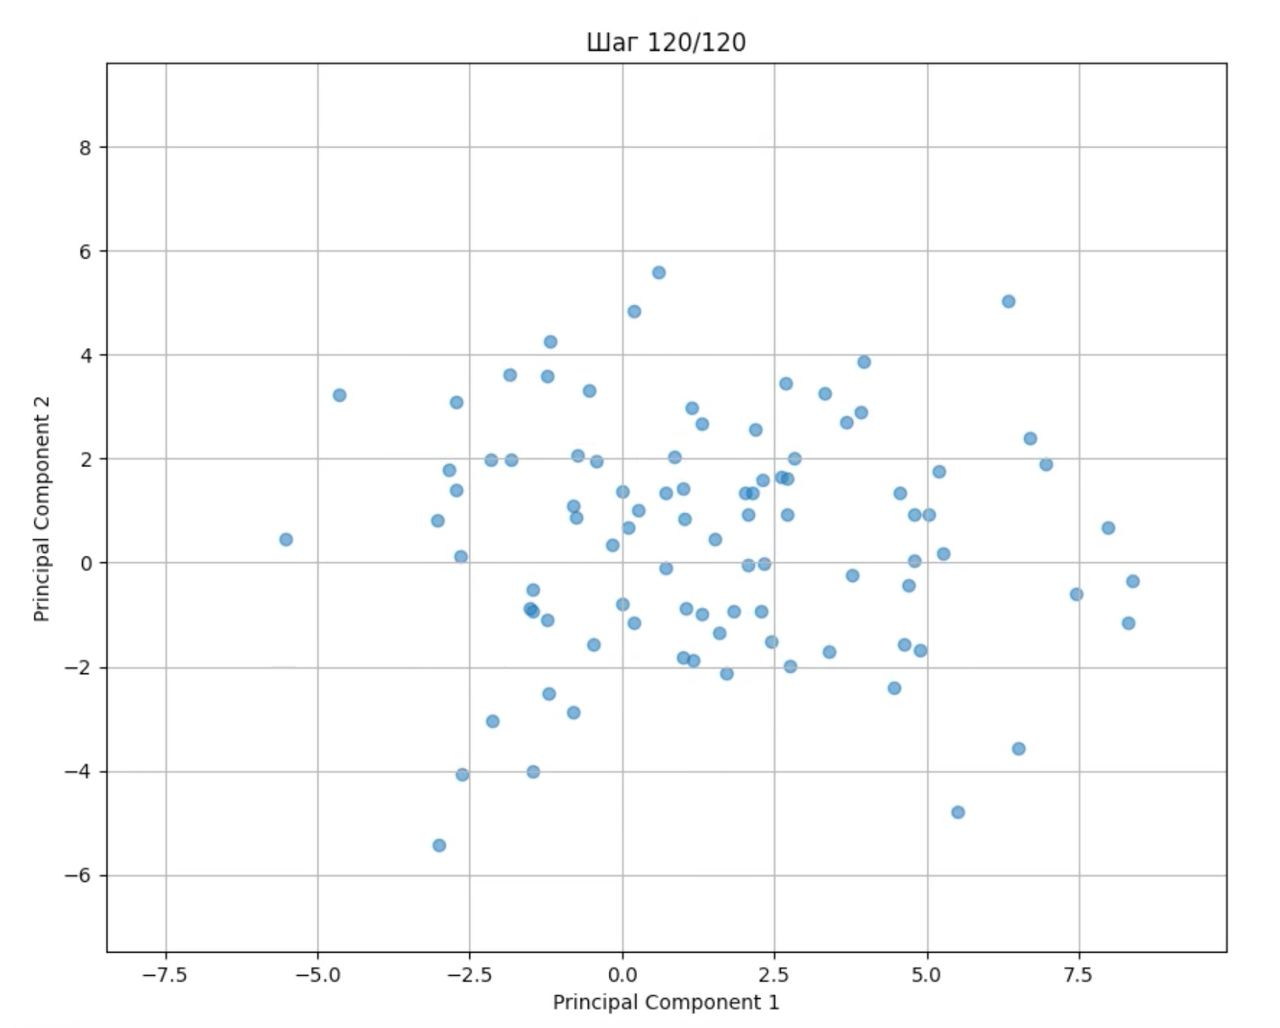
\includegraphics[width=0.38 \textwidth]{user_stable_2.png}

    \end{itemize}
    
\item {Скрытая петля отрицательной обратной связи }
\end{frame}

\begin{frame}{Анализируем результаты}
\begin{itemize}

\item В ходе экспериментов была получена явная зависимость от времени, которую если не учитывать, то система будет либо сходится к стационарной, либо будет происходить data drift только малой части данных

\item От количества информации в данных зависит возникновение петли. Это легко получить, используя разные размеры эмбеддингов для модели рекомендации, а также изменяя преобзования эмбеддингов

\end{itemize}
\end{frame}

\begin{frame}{Вывод}
\begin{itemize}

\item Мы получили качественное правило появления петли обратной связи

\item Смогли получить петлю на реальных данных

\item в дальнейшем будем исследовать сходимость многомерных распределений, а также рассматривать $KL$-дивергенцию между соседними распределениями
\end{itemize}
\end{frame}

\begin{frame}{Список литературы}
    \scriptsize
    \begin{thebibliography}{9}
        \bibitem{1} Wenlong Sun et al. \textit{Debiasing the Human-Recommender System Feedback Loop in
Collaborative Filtering }, 2019.
        \bibitem{2} Karl Krauth et al. \textit{Breaking Feedback Loops in Recommender Systems with Causal Inference}, 2022.
        \bibitem{3} Anton Khritankov. \textit{Positive feedback loops lead to concept drift in machine learning systems}, 2023.


    \end{thebibliography}
\end{frame}

\end{document}